\subsubsection{Fifth article}
 Next, we move on to the article \textit{"Domain Adaptation with Invariant Representation Learning: What Transformations to Learn?"} written by Stojanov, Petar, et al. \cite{stojanov2021domain} The researchers focus on the conditional shift scenario, where the data-generating process is utilized to (\textbf{i}) explain why two distinct encoding functions are required to infer the latent representation, (\textbf{ii}) improve an implementation of these functions, and (\textbf{iii}) impose meaningful structure on the latent representation $Z$ to increase prediction accuracy in the target domain.

\begin{figure}[H]
    \centering
    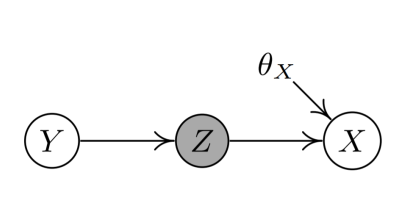
\includegraphics[width=0.5\textwidth]{Figures/From articles/DA_transforms.png}
    \caption{Data-generating process under conditional shift}
    \label{fig: DA_transf}
\end{figure}

Let's consider the data-generating process shown in the Figure \ref{fig: DA_transf} to understand what information is required for learning. The label $Y$ is generated first from its prior distribution $P(Y)$. Then, the invariant representation $Z$ is generated from $Y$ through $P(Z|Y)$, and $X$ is generated from $P(X|Z; \theta_X)$, where $\theta_X$ represents the changing parameters of $P(X|Y)$ across domains. We can consider $Z$ as a latent representation of our data. The variable $\theta_X$ may correspond to environment-specific changes that are irrelevant for predicting the class $Y$. Generally speaking, $Z$ is conditionally dependent on $\theta_X$ given $X$, although they may be marginally independent. Therefore, to recover $Z$ given $X$, the information of $\theta_X$ should also be considered in the transformation (see detailed in the article to understand clearly how authors measure the influence of $\theta_X$). The authors made two key observation associated with the data-generating process. Firstly, the encoder function $\phi$ requires $\theta_X$ as an input in addition to X. Secondly, assuming that $\theta_X$ has minimal influence on the relationship between $X$ and $Z$, allowing us to use a single encoder $\phi(X, \theta_X)$ instead of two separate encoders. A decoder function $\widetilde{\phi}$ that restricts the influence of $\theta_X$, acting as a regularizer on the encoder $\phi$, in order to retain important semantic information.

\begin{figure}[H]
    \centering
    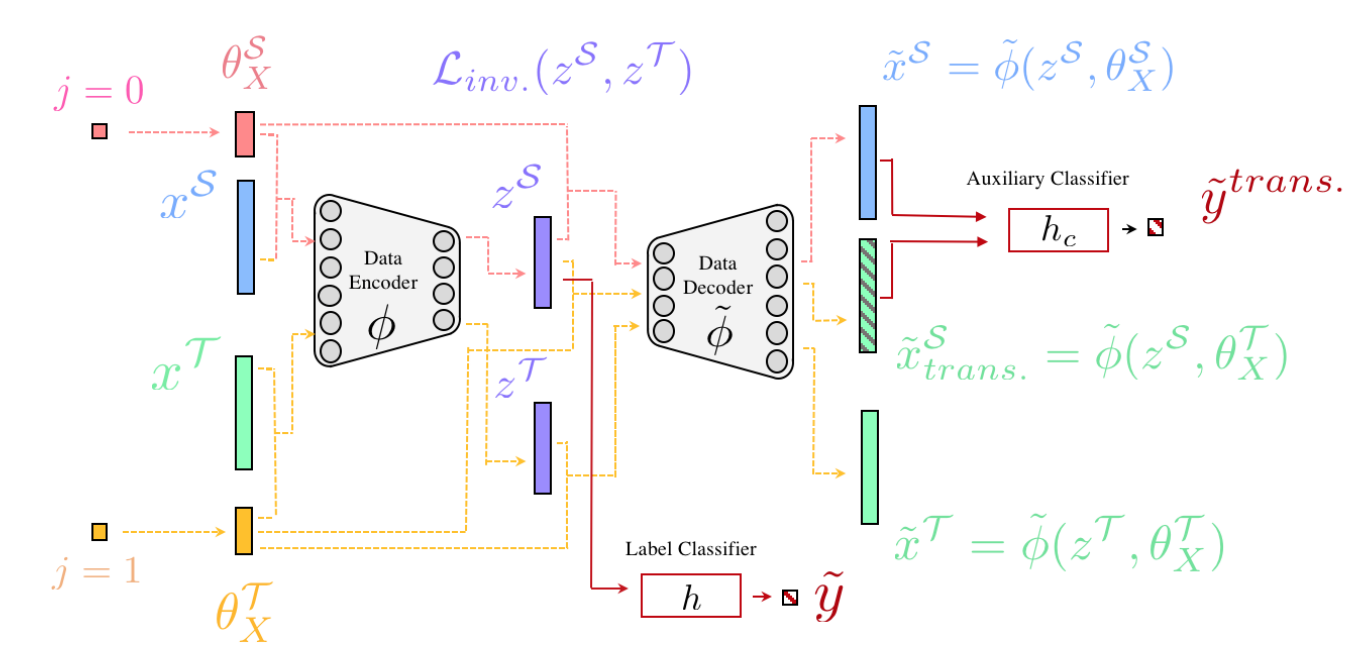
\includegraphics[width=0.85\textwidth]{Figures/From articles/DA_cnn.png}
    \caption{Autoencoder framework used in this article}
    \label{fig: DA_cnn}
\end{figure}

Thus, the authors proposed a domain-adaptation network, which is shown in the Figure \ref{fig: DA_cnn}, where $\theta_X \in \{\theta_X^S, \theta_X^T\}$ parameters for source and target domains respectively. 